\documentclass[10.5pt,a4paper]{article}
\usepackage[margin=18mm,top=18mm,bottom=20mm]{geometry}
\usepackage[T1]{fontenc}
\usepackage[utf8]{inputenc}
\usepackage{lmodern}
\usepackage{microtype}
\usepackage{graphicx}
\usepackage{booktabs}
\usepackage{tabularx}
\usepackage{longtable}
\usepackage{array}
\usepackage{xcolor}
\usepackage{enumitem}
\usepackage{listings}
\usepackage{fancyhdr}
\usepackage{hyperref}
\usepackage{titlesec}
\usepackage{caption}
\usepackage{lastpage}
\usepackage{amsmath}
\usepackage{float}
\usepackage{url}

\definecolor{ink}{HTML}{17212B}
\definecolor{muted}{HTML}{566574}
\definecolor{green}{HTML}{1F7A5A}
\definecolor{blue}{HTML}{2D6CA2}
\definecolor{amber}{HTML}{B86F1D}
\definecolor{red}{HTML}{A33A3A}
\definecolor{palegreen}{HTML}{EAF6EF}
\definecolor{paleblue}{HTML}{EDF5FA}
\definecolor{palered}{HTML}{FFF2EE}
\definecolor{line}{HTML}{CBD4DC}
\hypersetup{colorlinks=true,linkcolor=blue,urlcolor=blue,citecolor=green,pdfauthor={Tom Klootwijk UGTS-KC},pdftitle={UGTS-KC 4.1 POCO X7 Pro Spatial Seed Native}}
\setlength{\parindent}{0pt}
\setlength{\parskip}{5pt}
\setlist[itemize]{leftmargin=5mm,itemsep=2pt,topsep=3pt}
\setlist[enumerate]{leftmargin=6mm,itemsep=2pt,topsep=3pt}
\titleformat{\section}{\Large\bfseries\color{ink}}{}{0pt}{}[\vspace{1pt}\color{line}\titlerule]
\titleformat{\subsection}{\large\bfseries\color{green}}{}{0pt}{}
\titleformat{\subsubsection}{\normalsize\bfseries\color{blue}}{}{0pt}{}
\captionsetup{font=small,labelfont=bf,textfont=it,justification=centering}
\pagestyle{fancy}
\fancyhf{}
\fancyhead[L]{\small\color{muted}UGTS-KC 4.1 Spatial Seed Native}
\fancyhead[R]{\small\color{muted}POCO X7 Pro source handoff}
\fancyfoot[L]{\small\color{muted}Tom Klootwijk edition}
\fancyfoot[R]{\small\color{muted}Page \thepage\ of \pageref{LastPage}}
\renewcommand{\headrulewidth}{0.4pt}
\renewcommand{\footrulewidth}{0.4pt}
\setlength{\headheight}{14pt}

\lstdefinestyle{shell}{
  basicstyle=\ttfamily\small,
  backgroundcolor=\color{paleblue},
  frame=single,
  rulecolor=\color{line},
  breaklines=true,
  columns=fullflexible,
  keepspaces=true,
  showstringspaces=false,
  xleftmargin=3mm,
  xrightmargin=3mm,
  aboveskip=6pt,
  belowskip=6pt
}
\lstset{style=shell}

\newcommand{\pass}{\textcolor{green}{\textbf{PASS}}}
\newcommand{\deferred}{\textcolor{amber}{\textbf{CODEX/DEVICE}}}
\newcommand{\risk}{\textcolor{red}{\textbf{NOT CLAIMED}}}
\newcommand{\filepath}[1]{\texttt{\detokenize{#1}}}
\newcommand{\hashline}[1]{\par\small\texttt{#1}\normalsize\par}

\begin{document}

% Cover
\begin{titlepage}
\pagecolor{ink}\color{white}
\vspace*{16mm}
{\Huge\bfseries UGTS-KC 4.1\par}
\vspace{3mm}
{\LARGE\bfseries POCO X7 Pro Spatial Seed Native\par}
\vspace{7mm}
{\large Camera2 + IMU capture, event verification, deterministic ledger and KSEED storage\par}
\vspace{17mm}
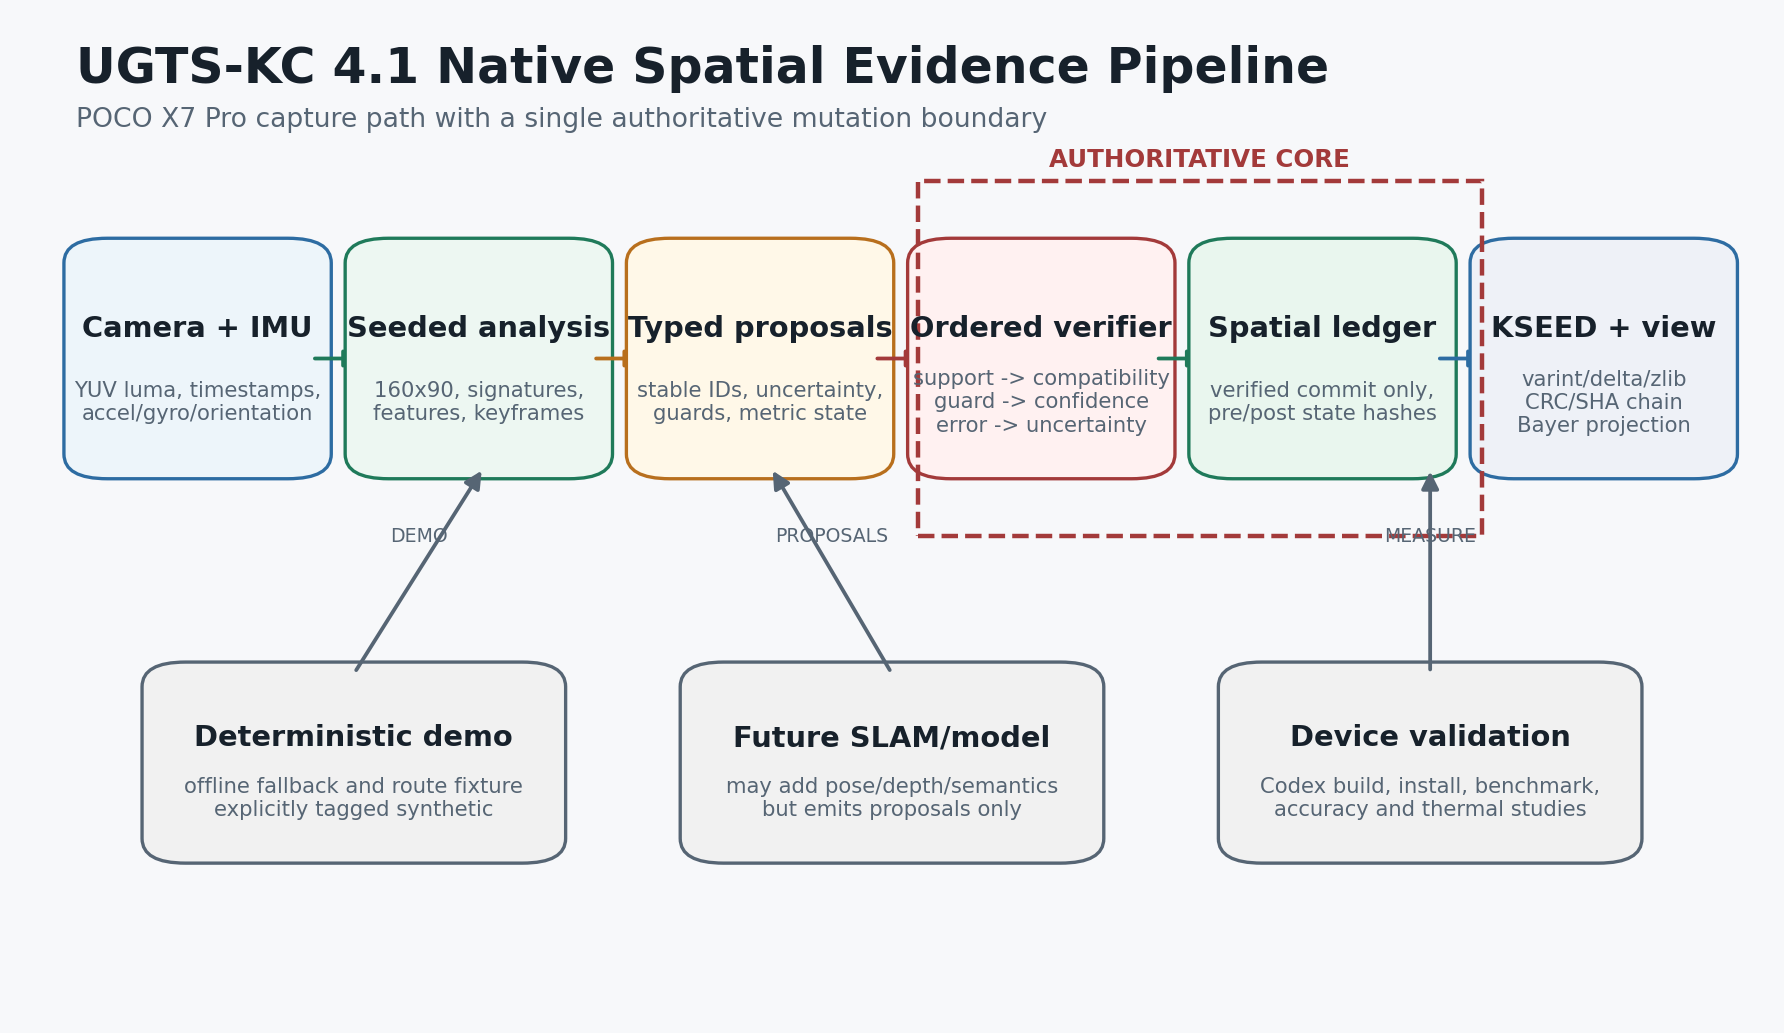
\includegraphics[width=\textwidth]{../diagrams/architecture_native_4_1.png}
\vfill
\begin{tabularx}{\textwidth}{>{\bfseries\color{white}}l X}
Release & 4.1.0 source handoff\\
Named target & POCO X7 Pro 12 GB, arm64-v8a\\
Base substrate & UGTS-KC 4.0 Spatial Evidence Ledger\\
Native baseline & UGTS-KC K-Kij-T / Grove 3.9.2\\
Storage & KSEED 4.1 seed plus measured evidence deltas\\
Build status & Source validated; Android SDK/NDK build and physical device test deferred to Codex\\
Prepared & 28 August 2026\\
\end{tabularx}
\vspace{10mm}
{\small\color{white!75}This report accompanies the complete source ZIP. It does not claim a newly built APK, physical-phone benchmark, complete SLAM system, safety certification, or production signing.}
\end{titlepage}
\nopagecolor\color{ink}

\tableofcontents
\clearpage

\section{Executive delivery statement}

UGTS-KC 4.1 completes the Android-native implementation that UGTS-KC 4.0 deliberately deferred. The active project begins from the attached, working 3.9.2 NativeActivity/Gradle/CMake pattern and replaces game-scene authority with the 4.0 spatial observation, ordered verification, deterministic commit, lineage and replay boundary.

The deliverable is intended for Codex to compile and deploy. It includes a complete Android Studio/Gradle project, portable C++ core, host tests, deterministic KSEED fixture, retained 4.0 Python reference, retained source-only 3.9.2 Android baseline, build/deploy/pull scripts, format and authority contracts, validation records, manifests and checksums.

\begin{table}[H]
\centering
\begin{tabularx}{\textwidth}{>{\bfseries}p{38mm} X p{28mm}}
\toprule
Deliverable element & Implemented content & Status\\
\midrule
Android native app & NativeActivity, Camera2 NDK, Media NDK image reader, NDK sensors, EGL/GLES3, touch and key input & \pass\\
POCO target & arm64-only flavor, device/GPU/RAM hints, 120 Hz request, 30 fps capture policy, thermal tiers & \pass\\
Spatial authority & typed proposals, ordered gates, stable IDs, ledger commit, pre/post state hashes & \pass\\
Seed storage & KSEED 4.1 delta/varint/zlib/CRC32/SHA-256 chain, no raw frames by default & \pass\\
Portable validation & 23 host tests, independent inspector, deterministic fixture and corruption detection & \pass\\
Android compilation & Requires SDK 36, NDK 29.0.14206865 and CMake 3.22.1 on Codex build host & \deferred\\
Physical POCO run & Install, camera negotiation, latency, thermal, battery and accuracy measurement & \deferred\\
\bottomrule
\end{tabularx}
\caption{Release status is separated into completed source evidence and deferred device evidence.}
\end{table}

\subsection{Key design decision}

The app stores a \textbf{seed plus evidence deltas}. The seed recreates deterministic sample schedules, stable identifiers, synthetic fixtures and procedural display choices. It does not recreate unstored real-world photons. Measured luma/IMU summaries, sparse feature values, accepted event data, uncertainty and hashes remain in the file. This boundary delivers real compression without making an impossible seed-only reconstruction claim.

\section{Source lineage and version promotion}

\subsection{UGTS-KC 4.0 authority base}

The 4.0 substrate defines the canonical path:

\begin{center}
\texttt{capture profile + observation -> support -> compatibility -> guard/error/uncertainty -> verified proposal -> deterministic commit -> hashes/lineage -> replay/export}
\end{center}

The retained \filepath{substrate/ugts_kc4/} namespace and 4.0 JSON schema remain in the package as a readable reference oracle. Native records mirror its distinction between observation and authority: callbacks and models propose; the verifier and ledger commit.

UGTS-KC 4.0 archive SHA-256:
\hashline{7ce064e5e4e2bb6b43d86f191db21111aab823771cbc1461413377a3c675d6d8}

UGTS-KC 4.0 report SHA-256:
\hashline{fe4a7dfbedb0163d90d22b4e6c5aef7e042f7342199a64eb3db3d76da1bdb1b4}

\subsection{UGTS-KC 3.9.2 native baseline}

The attached 3.9.2 project supplies the proven NativeActivity lifecycle, Gradle/CMake pins, arm64 POCO flavor, high-refresh request, device selection, adaptive quality shape and small native packaging approach. A source-only, unmodified reference copy is under \filepath{upstream/android_3_9_2_reference/}.

Attached 3.9.2 archive SHA-256:
\hashline{bd7f8aa7e5829f27020a859d9e16a8b2917017c171045fd75a1814a0cb6d4486}

The new app is not a rename of the game. It carries the working platform pattern forward while replacing the content path with Camera2/IMU observations, KSEED storage and the 4.0 ledger authority.

\subsection{Mechanism catalog}

Mechanisms M510--M569 are added as sixty contiguous implementation mechanisms. They cover capture, bounded buffering, IMU acquisition, seeded analysis, keyframe policy, 64-bit keys, verifier gates, ledger hashing, KSEED framing, integrity, app-private storage, Bayer presentation, thermal reduction and Codex promotion gates. The catalog is supplied as CSV and JSON.

\clearpage
\section{Native architecture}

\begin{figure}[H]
\centering
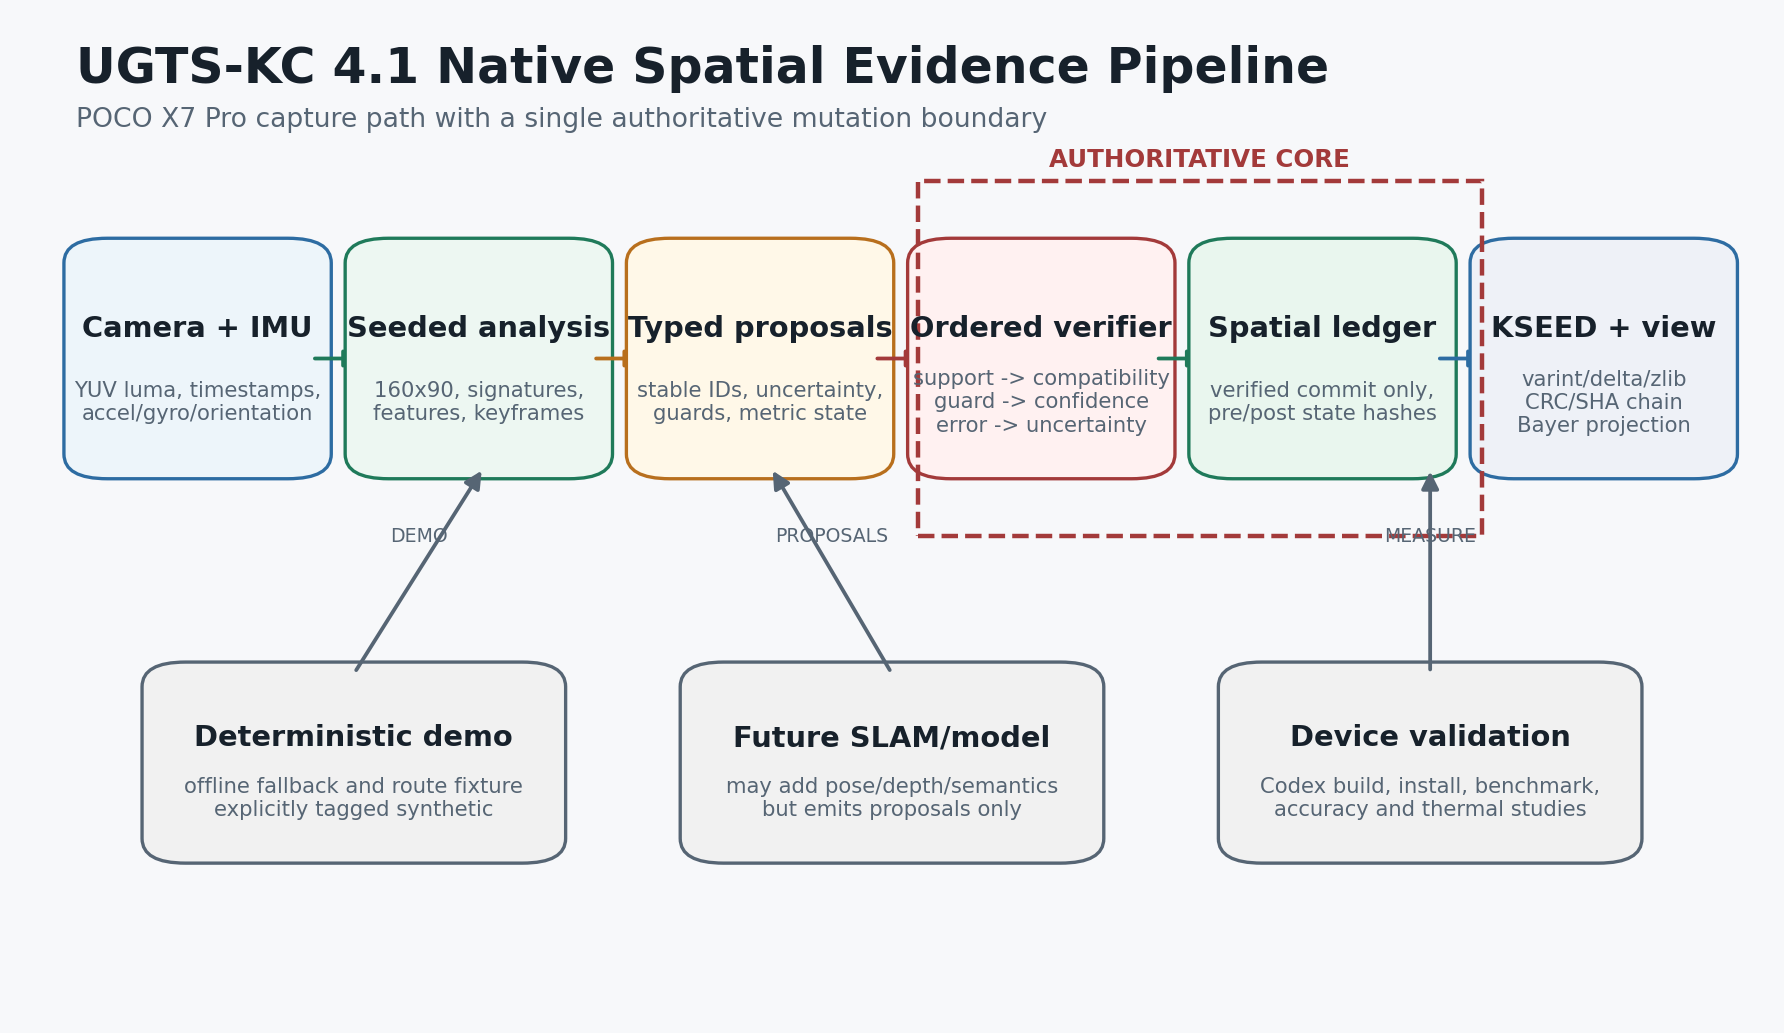
\includegraphics[width=\textwidth]{../diagrams/architecture_native_4_1.png}
\caption{The verifier and ledger form the only authoritative map mutation path.}
\end{figure}

\subsection{Lifecycle and bounded data movement}

The application uses \texttt{android.app.NativeActivity}; no Java or Kotlin runtime layer is needed. The main loop receives window/focus/input lifecycle callbacks through \texttt{android\_native\_app\_glue}.

Camera callbacks acquire the newest \texttt{YUV\_420\_888} frame, copy the Y plane into one mutex-protected buffer, and replace the previous unread frame. The implementation intentionally drops old frames rather than creating an unbounded queue. Sensor callbacks similarly keep only the latest accelerometer, gyroscope and rotation-vector state.

The engine consumes frames at a thermal-policy rate. It downsamples to a fixed 160x90 analysis field, computes a luma signature and spatially distributed features, applies a keyframe gate, creates typed proposals, verifies them, commits accepted events and appends compact records.

\subsection{Authority boundary in code}

\begin{itemize}
\item \filepath{camera_ndk.cpp} and \filepath{imu_ndk.cpp}: measured input only.
\item \filepath{core/feature_extractor.cpp}: deterministic candidates only.
\item \filepath{core/pipeline.cpp}: typed proposal adaptation.
\item \filepath{core/verifier.cpp}: reason-coded ordered acceptance gates.
\item \filepath{core/ledger.cpp}: the sole accepted-state mutation boundary.
\item \filepath{core/kseed_codec.cpp}: deterministic storage and integrity.
\item \filepath{renderer_bayer.cpp}: non-authoritative projection only.
\end{itemize}

A future visual-inertial estimator or distilled transformer can be inserted before proposal adaptation. It may add pose, depth, normal, semantic, route or change proposals with calibrated uncertainty. It may not call unchecked map mutation.

\section{POCO X7 Pro profile}

The named flavor is \texttt{pocoX7ProRelease}, application ID \texttt{nl.tomklootwijk.ugtskc.spatial.poco}, and ABI \texttt{arm64-v8a}. Runtime selection verifies POCO model/device hints, a Mali-G720 renderer hint and a reported-memory floor before selecting the 12 GB profile.

\begin{table}[H]
\centering
\begin{tabularx}{\textwidth}{>{\bfseries}p{42mm} X}
\toprule
Policy & Requested value\\
\midrule
Camera stream & rear \texttt{YUV\_420\_888}, nearest available to 1280x720\\
Capture cadence & 30 fps request\\
Analysis field & 160x90 luma\\
Feature budget & up to 128 candidates per retained keyframe\\
Presentation & 120 Hz request through \texttt{ANativeWindow\_setFrameRate}, OS/display permitting\\
Display backend & OpenGL ES 3.0 fullscreen triangle and one R8 texture\\
Storage & KSEED seed-plus-deltas, 128 KiB chunk target, no raw frames\\
Network & no Internet permission declared\\
\bottomrule
\end{tabularx}
\caption{Policies are requests, not guaranteed device measurements.}
\end{table}

\begin{figure}[H]
\centering
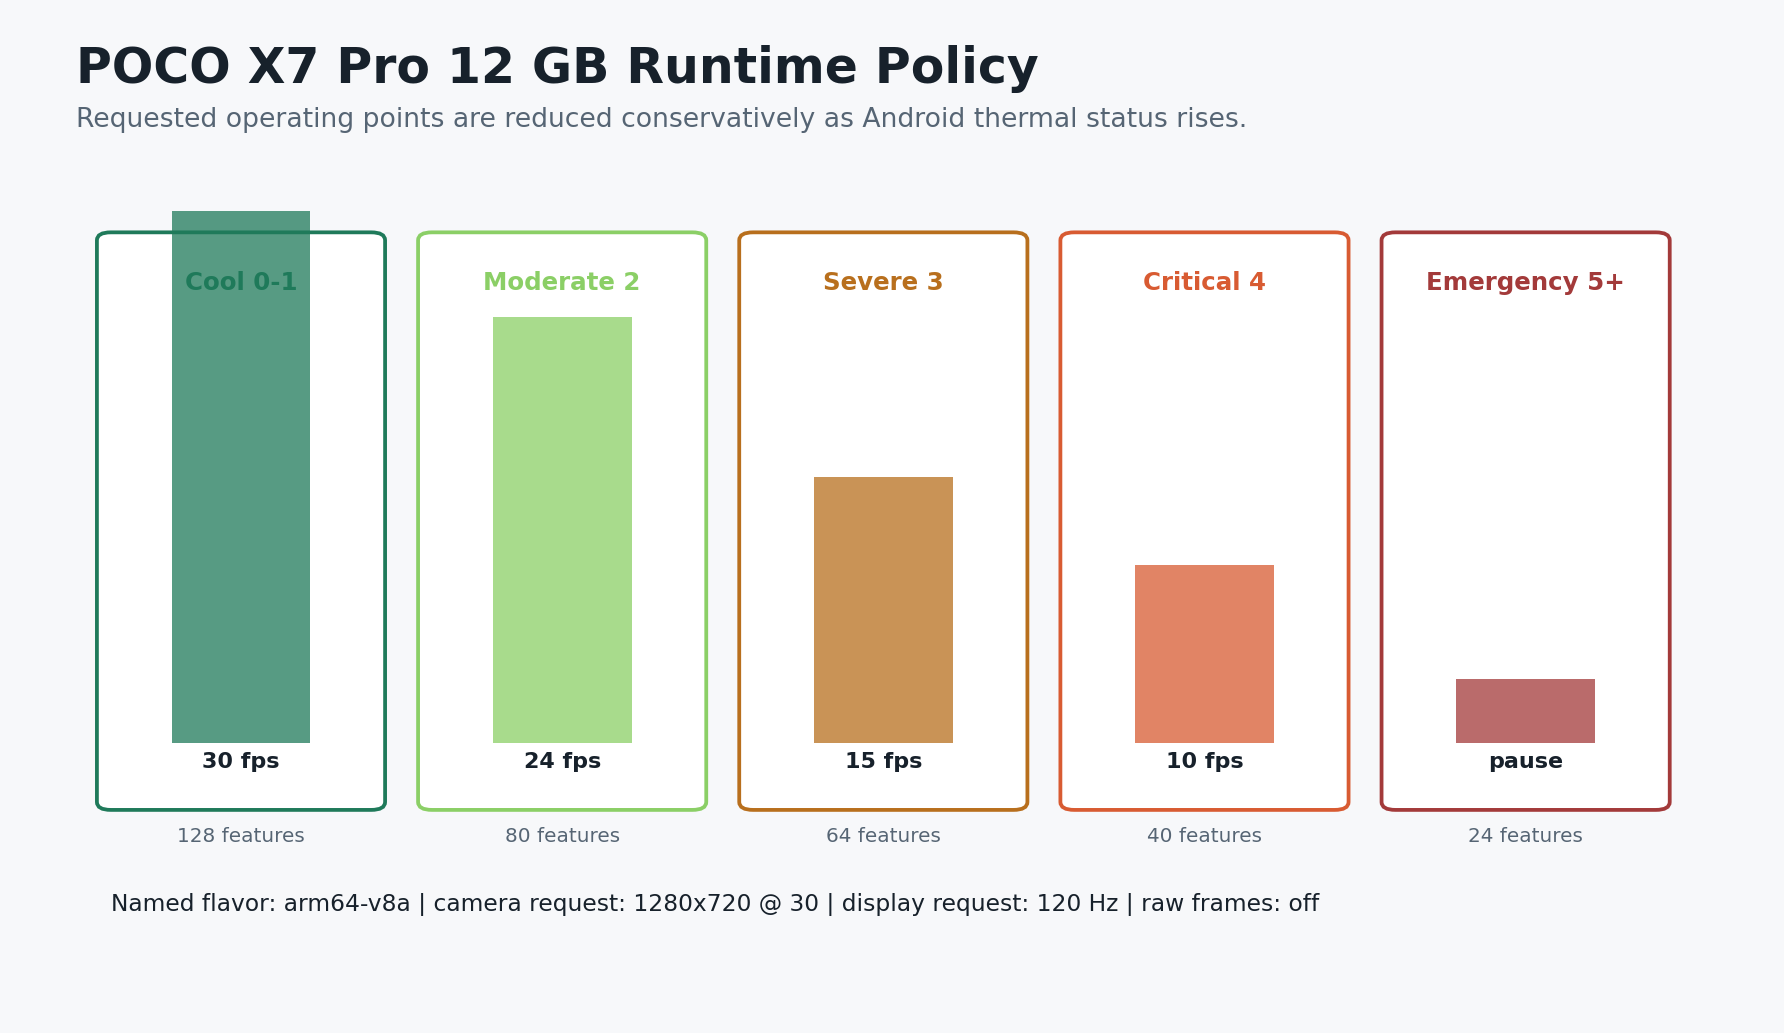
\includegraphics[width=0.94\textwidth]{../diagrams/poco_runtime_4_1.png}
\caption{Thermal status reduces processing rate and feature budget; severe status pauses authoritative capture.}
\end{figure}

Device-specific optimization does not relax verifier thresholds. A thermal policy change is itself recorded as an event so a later reviewer can see when capture conditions changed.

\section{Seeded feature and keyframe path}

The analysis path uses only the luma plane by default. This minimizes memory bandwidth and avoids retaining sensitive raw color frames.

\subsection{Deterministic extraction}

Each camera frame is resampled to 160x90. The extractor computes:

\begin{itemize}
\item mean and standard deviation of luma;
\item an 8x8 block-mean comparison signature, stored as 64 bits;
\item horizontal/vertical gradient magnitude;
\item grid-distributed candidate selection;
\item SplitMix64 seed tie-breaking;
\item Morton ordering for compact coordinate deltas;
\item a 64-bit camera-ray key reconstructed from pixel, frame and profile dimensions.
\end{itemize}

The seed makes candidate tie-breaking and stable identities reproducible. It does not manufacture measurements: intensity, gradient, IMU and event values still come from retained data.

\subsection{Keyframe gate}

The first frame is retained. Later frames must pass a minimum interval and then satisfy visual signature change, orientation change or a maximum interval. A minimum feature count prevents low-information frames from being promoted solely by minor change. Thermal tiers reduce the feature budget and effective processing rate.

\begin{figure}[H]
\centering
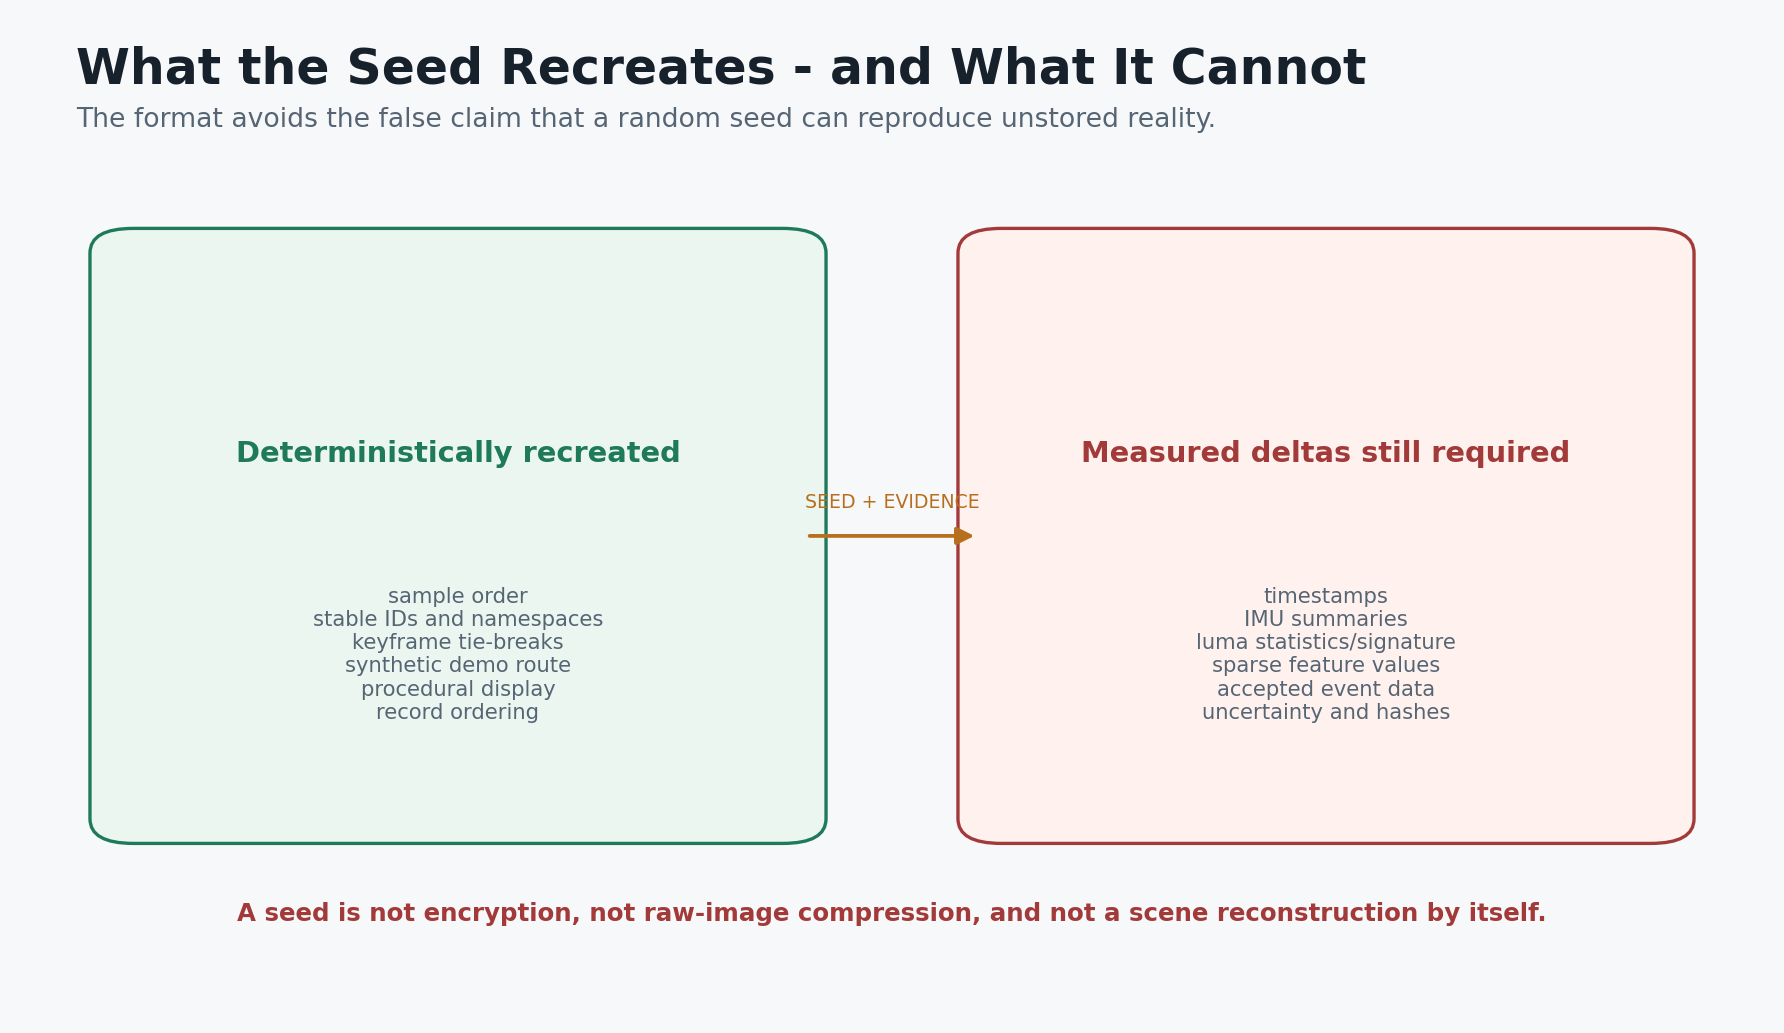
\includegraphics[width=0.94\textwidth]{../diagrams/seed_boundary_4_1.png}
\caption{The session seed and measured deltas have distinct roles.}
\end{figure}

\clearpage
\section{KSEED 4.1 compact storage}

\begin{figure}[H]
\centering
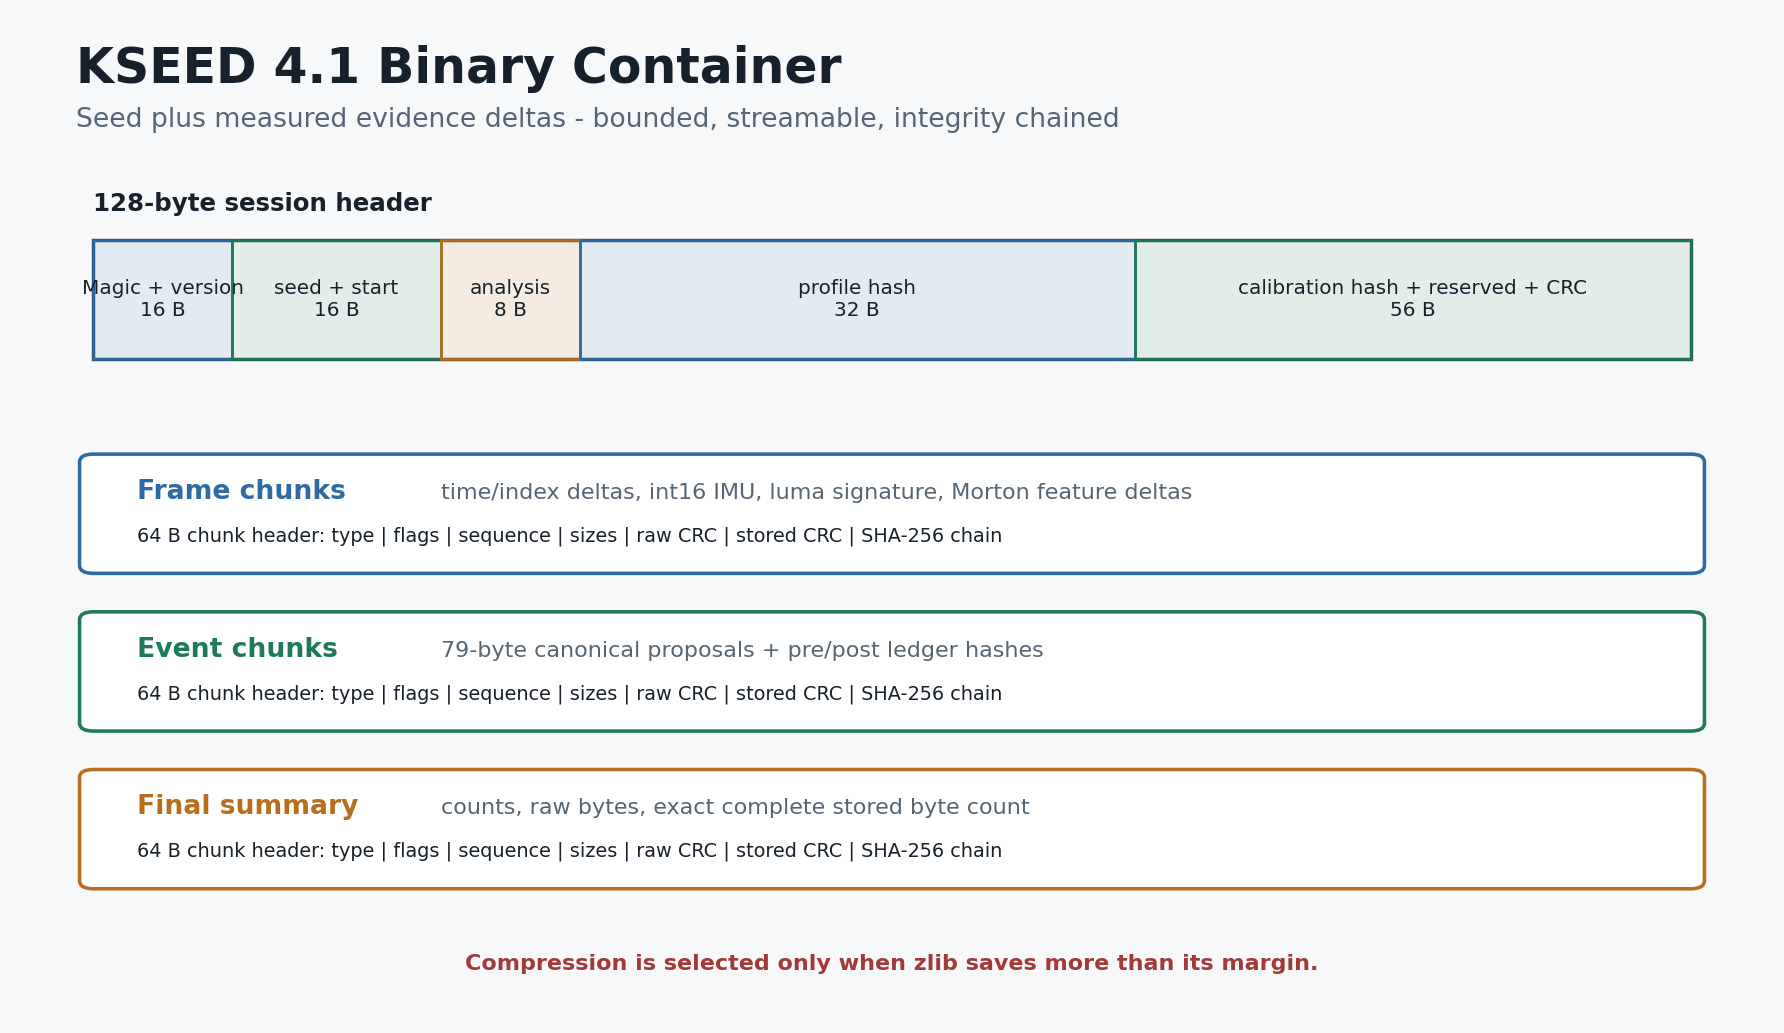
\includegraphics[width=\textwidth]{../diagrams/kseed_layout_4_1.png}
\caption{KSEED is a streamable sequence of independently checked chunks.}
\end{figure}

\subsection{Session header}

The 128-byte file header declares version, storage mode, seed, start time, analysis dimensions, requested capture rate, feature budget, capture-profile SHA-256 and calibration-descriptor SHA-256. A CRC32 over bytes 0--123 detects header corruption.

\subsection{Chunk integrity}

Every 64-byte chunk header declares type, flags, sequence, record count, decoded/stored lengths and two CRC32 values. The chain is:

\[
H_i = \operatorname{SHA256}(H_{i-1} \parallel C_i[0:32] \parallel P_i)
\]

where the initial predecessor is \(\operatorname{SHA256}(\texttt{"KSEED41-CHAIN"})\), \(C_i\) is the chunk header and \(P_i\) is the stored payload. Replay stops at the first framing, CRC or chain failure.

\subsection{Compression rules}

Frame and event records use delta timestamps, delta frame indices, int16 inertial quantization, Morton-coordinate deltas and base-128 varints. A payload is zlib-compressed at \texttt{Z\_BEST\_SPEED} only when compressed bytes plus a 16-byte margin are smaller than the raw payload. This prevents compression expansion.

The final 60-byte summary stores session counts, raw input bytes and the exact predicted complete file size. The reader checks that \texttt{stored\_bytes} equals the actual file length.

\subsection{Synthetic fixture result}

The checked-in deterministic fixture contains 300 generated 320x180 luma frames. It retains 63 keyframes and 592 events, and stores 17,280,000 raw input bytes as a 79,053-byte KSEED file.

\begin{figure}[H]
\centering
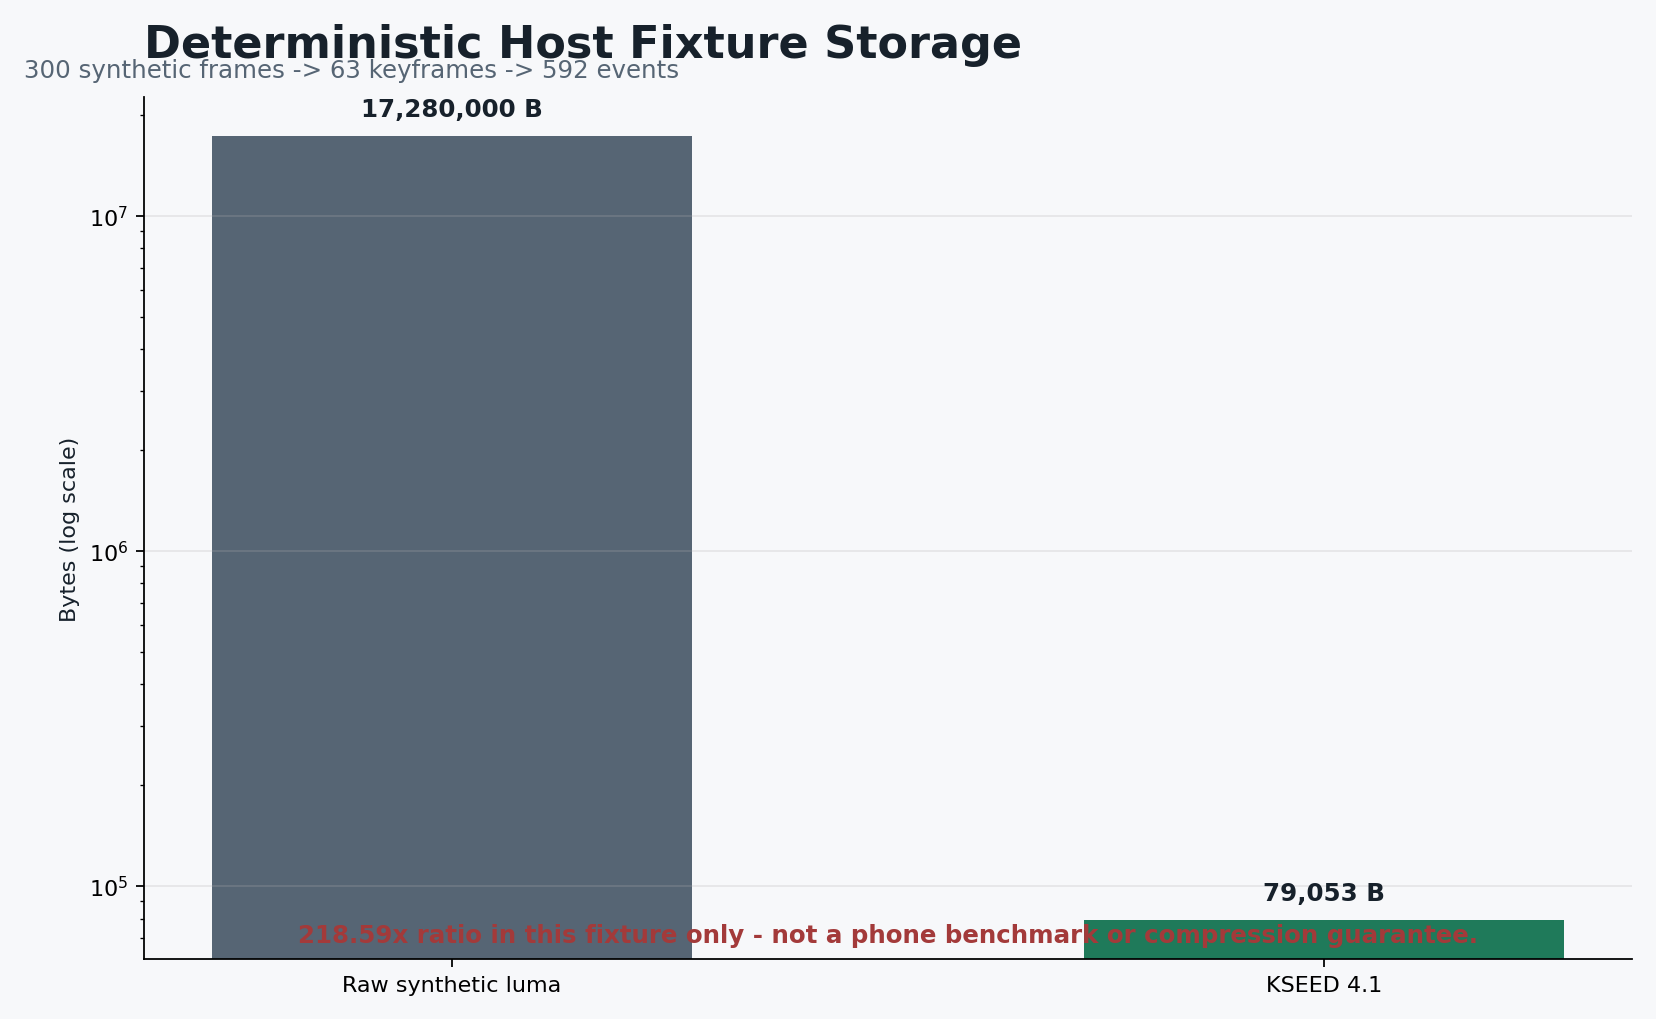
\includegraphics[width=0.82\textwidth]{../diagrams/storage_fixture_4_1.png}
\caption{The 218.59x ratio is a deterministic host fixture, not a phone benchmark or compression guarantee.}
\end{figure}

Current fixture SHA-256:
\hashline{b70010f3435608f6e1baa7dc4bd04edb151385413383130b45f529275bfe008c}

\section{Verification and ledger semantics}

The native verifier follows the 4.0 operation order. A proposal is rejected when any required gate fails:

\begin{enumerate}
\item identifier validity;
\item local support;
\item semantic/topological compatibility;
\item accepted guard class;
\item confidence floor;
\item numeric error margin;
\item maximum uncertainty;
\item metric availability when the event requires metric meaning.
\end{enumerate}

Every accepted event receives a sequence, canonical proposal bytes, pre-state hash and post-state hash. Stable node identity is independent of coordinates and may accumulate evidence without coordinate-only aliasing. Route nodes and route edges have separate identities, uncertainty and passability fields.

\subsection{Synthetic fallback isolation}

If camera permission or camera startup fails, the app remains testable by generating a deterministic luma pattern and route fixture. The screen explicitly shows \texttt{DEMO}. Synthetic proposals set tag bit 31. This permits offline UI/ledger/storage validation while preserving the evidence boundary.

\section{Bayer display and interaction}

The renderer uses a fullscreen triangle and a single \texttt{GL\_R8} texture. An 8x8 ordered Bayer threshold maps luma to four display levels with a mode-specific tint. The display path contains no ray tracing, no ray marching and no dense 3D scene. Ordinary GPU rasterization is used only to put the already-derived projection on the screen.

The three modes are:

\begin{itemize}
\item \textbf{Camera}: luma preview, seeded feature marks and recording status.
\item \textbf{Map Demo}: a deterministic route fixture generated from the seed, visibly marked demo.
\item \textbf{Ledger}: event/rejection counts and a visualization derived from the current state hash.
\end{itemize}

Tap or Volume Up toggles recording. Horizontal swipe rotates modes. App-private sessions are written beneath the NativeActivity internal files directory in \filepath{sessions/}.

\section{Codex build and deploy handoff}

\subsection{Pinned toolchain}

\begin{table}[H]
\centering
\begin{tabular}{ll}
\toprule
Component & Pin\\
\midrule
Android Gradle Plugin & 8.13.2\\
Gradle & 8.13\\
compileSdk / targetSdk & 36 / 36\\
minSdk & 26\\
Android NDK & 29.0.14206865\\
CMake & 3.22.1\\
Language & C++20\\
\bottomrule
\end{tabular}
\end{table}

The custom Unix \texttt{gradlew} bootstrap downloads the official Gradle 8.13 binary and checks SHA-256 \texttt{20f1b117...0aed78} before use.

\subsection{Build}

\begin{lstlisting}
cd android_project
export ANDROID_SDK_ROOT="$HOME/Android/Sdk"
./gradlew --no-daemon clean :app:assemblePocoX7ProRelease
\end{lstlisting}

Expected output:

\begin{lstlisting}
android_project/app/build/outputs/apk/pocoX7Pro/release/
  app-pocoX7Pro-release.apk
\end{lstlisting}

\subsection{Install and launch}

\begin{lstlisting}
APP_ID=nl.tomklootwijk.ugtskc.spatial.poco
APK=android_project/app/build/outputs/apk/pocoX7Pro/release/\
app-pocoX7Pro-release.apk
adb install -r "$APK"
adb shell pm grant "$APP_ID" android.permission.CAMERA || true
adb shell am start -n "$APP_ID/android.app.NativeActivity"
adb logcat -s UGTS-KC-4.1:* AndroidRuntime:E
\end{lstlisting}

\subsection{Pull and inspect sessions}

The owner-device release is deliberately debug-key signed and debuggable for this handoff. That allows \texttt{run-as}; it is not a public-distribution configuration.

\begin{lstlisting}
APP_ID=nl.tomklootwijk.ugtskc.spatial.poco
mkdir -p pulled_sessions
adb exec-out run-as "$APP_ID" sh -c \
  'cd files && tar cf - sessions' | tar xf - -C pulled_sessions
python3 tools/kseed_inspect.py \
  pulled_sessions/sessions/<session>.kseed --json
\end{lstlisting}

Complete commands and the mandatory device-validation record are in \filepath{docs/CODEX_BUILD_AND_DEPLOY.md}.

\section{Validation results}

\begin{figure}[H]
\centering
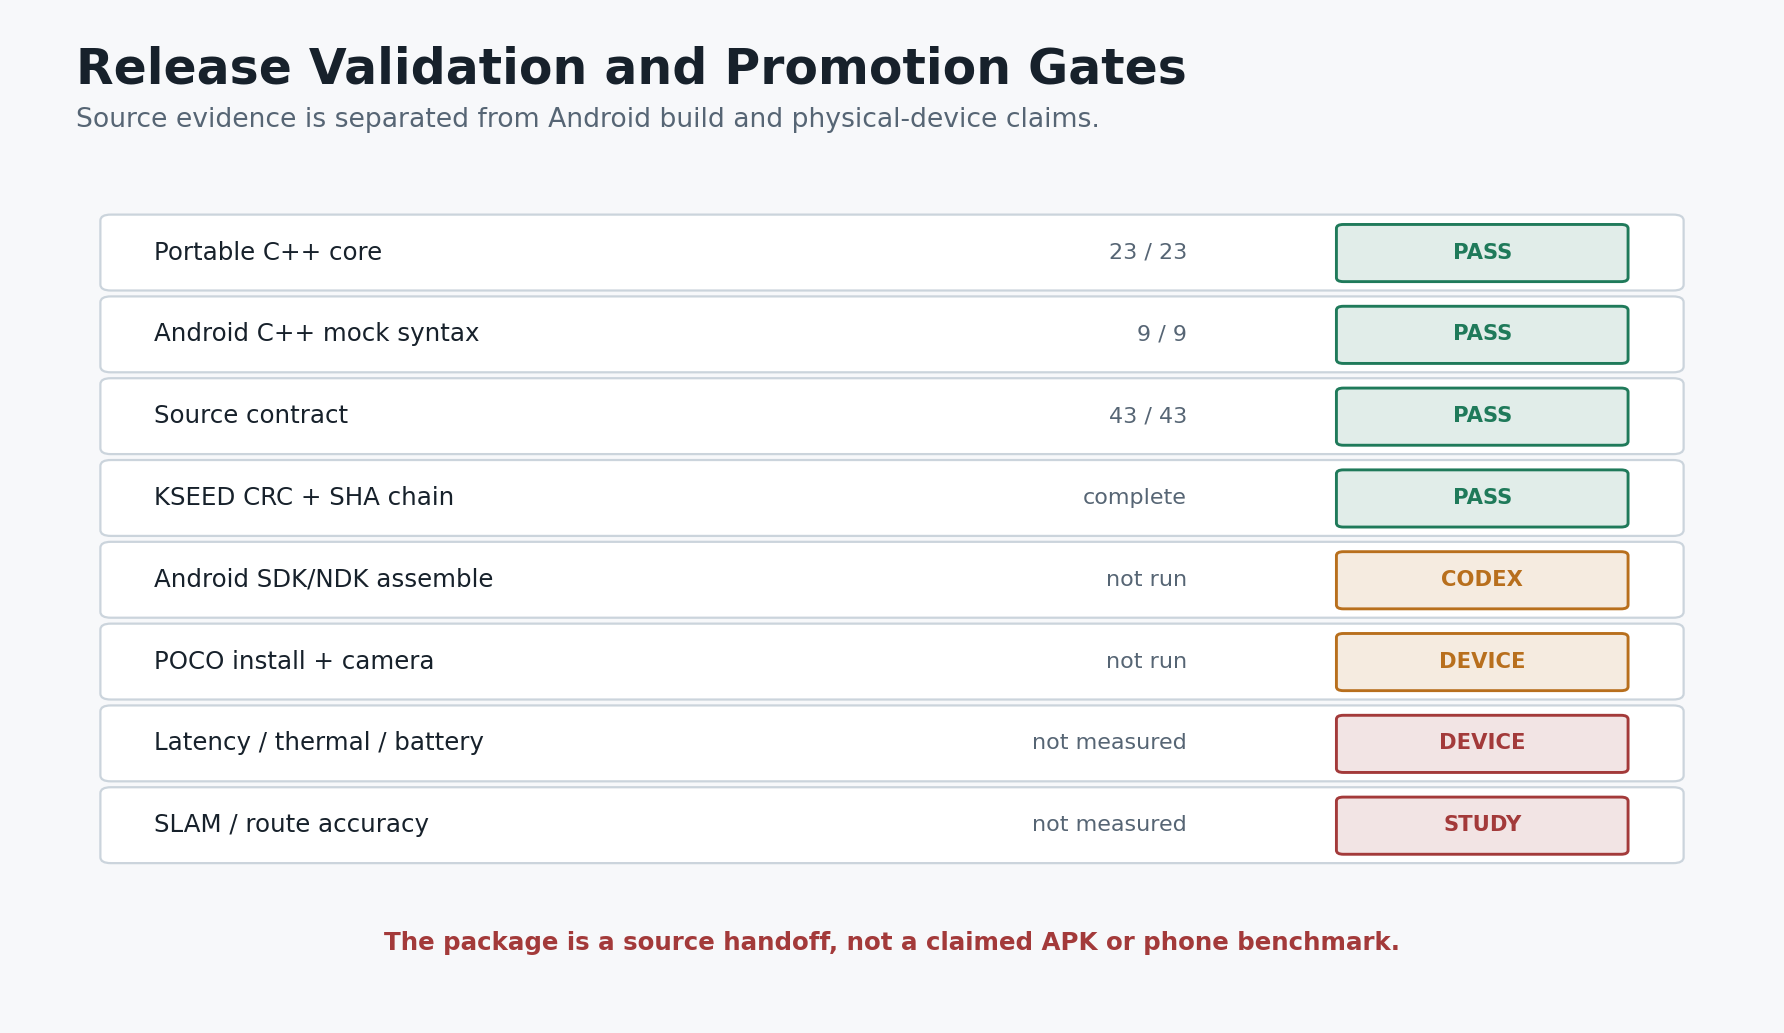
\includegraphics[width=0.94\textwidth]{../diagrams/validation_4_1.png}
\caption{Completed source checks are visually separated from promotion gates.}
\end{figure}

\subsection{Portable C++ core}

The host build compiles the same seed, keys, feature extraction, verifier, ledger, pipeline, SHA-256, CRC32, varint and KSEED sources used by Android. It passes 23 checks covering deterministic seeds, key packing, extraction, keyframe selection, verifier acceptance/rejection, ledger hashing, route commit, KSEED write/read, exact final size, optional thumbnails and corruption detection.

\subsection{Independent KSEED inspector}

A separate Python reader verifies file/header version, header CRC, stored CRC, zlib decode, decoded CRC, chunk order, SHA-256 chain and final summary. It reports complete integrity for the fixture.

\subsection{Android source checks}

Nine Android-specific translation units pass a C++20 syntax check against a mock surface for the NDK interfaces. A 43-check source contract confirms Gradle/toolchain pins, product flavors, manifest permissions, native libraries, Camera2/YUV path, NDK sensors, verifier/ledger authority, KSEED integrity, profile privacy, Bayer shader, upstream source hash and absence of build caches.

\subsection{What was not executed here}

The environment used to assemble this package did not contain the Android SDK/NDK and did not have a physical POCO X7 Pro attached. Therefore this report does not claim an APK, camera stream success, device FPS, memory use, thermal behavior, battery use, model accuracy or route correctness.

\section{Promotion gates and limitations}

Before describing the app as a validated scanner or operational spatial tool, Codex/device testing must record:

\begin{itemize}
\item exact phone model, RAM edition, OS build, GPU string and display mode;
\item selected camera ID, actual YUV dimensions and actual frame cadence;
\item p50/p95/p99 frame processing and storage latency;
\item dropped frames, peak memory and bytes per minute;
\item 5, 15 and 30 minute thermal and battery traces;
\item KSEED pull, independent integrity check and deterministic replay;
\item task-specific false/missed-event rates and route/change accuracy;
\item comparison against a conventional calibrated baseline.
\end{itemize}

The current real-camera path records sparse visual/inertial evidence but does not implement metric visual-inertial SLAM, dense depth, a distilled transformer, loop closure or certified topology recognition. The deterministic route map is a fixture, not a reconstruction of the camera scene. The architecture is prepared for these additions without weakening verification.

KSEED hashes detect changed bytes; they do not prove operator identity, truthful location, uncompromised hardware, external time, ownership or legal chain of custody. The seed is not encryption. Production distribution must replace debug signing, disable debugging and define retention/security policy.

\section{Package contents}

\begin{longtable}{>{\bfseries}p{42mm} p{115mm}}
\toprule
Path & Purpose\\
\midrule
\endfirsthead
\toprule
Path & Purpose\\
\midrule
\endhead
\filepath{android_project/} & Complete Codex-buildable NativeActivity project and active source.\\
\filepath{native/host_tests/} & Portable CMake tests and deterministic demo generator.\\
\filepath{substrate/} & Retained UGTS-KC 4.0 Python namespace, schema and contract.\\
\filepath{upstream/} & Source-only attached 3.9.2 Android reference plus source hashes.\\
\filepath{tools/} & Android build/deploy/pull, KSEED inspect, source contract and package verify tools.\\
\filepath{spec/} & KSEED binary format, Android authority contract, profile JSON and M510--M569 catalogs.\\
\filepath{examples/} & Verified synthetic KSEED, summary and route GeoJSON.\\
\filepath{validation/} & Host, inspector, syntax, compile and source-contract evidence.\\
\filepath{report/} & This PDF and editable LaTeX source.\\
\filepath{manifest/} & JSON/CSV inventory and readable package tree.\\
\filepath{checksums/} & SHA-256 release list.\\
\bottomrule
\end{longtable}

\section{References}

{\small
\begin{enumerate}[itemsep=0pt,topsep=1pt,parsep=0pt]
\item \textit{UGTS-KC 4.0 Spatial Evidence Ledger}, supplied project report and source package.
\item \textit{UGTS-KC K-Kij-T / Grove 3.9.2 Complete All Files}, supplied native Android baseline.
\item \textit{UGTS-KC Two Hands 3.0 Interactive Graphics Runtime}, stable identity, deterministic commit and projection boundaries.
\item \textit{UGTS-KC 3.6 and 3.6.2}, content-addressed definitions, bounded supports and 64-bit indexing discipline.
\item \textit{UGTS-KC 2.0 Expanded Substrate}, typed events, topology, routes, SE(3) and uncertainty foundations.
\item \textit{Unified Geometric Topological Substrate GPU-Native Addendum}, precision and GPU authority boundaries.
\item Android Developers, Android NDK Camera, Image Reader, Sensors, NativeActivity and build-tool documentation.
\item POCO official product specifications for POCO X7 Pro and MediaTek official Dimensity 8400 platform material, used only to select a requested device profile; physical runtime remains unverified in this release.
\end{enumerate}
}

\vfill
\begin{center}
\color{muted}\small
End of UGTS-KC 4.1 POCO X7 Pro Spatial Seed Native technical report.\\
The accompanying ZIP is the authoritative source handoff for Codex build and device deployment.
\end{center}

\end{document}
